\chapter{网页版式评分系统}
\label{chap:application}

网页版式评分系统是对人的审美能力的一种有限模仿。通过第\ref{chap:exp2}章中对视觉复杂度和视觉显著性分布的相关特征对美感的推测力的证实,用这些特征训练得到的模型即可以作为版式评分系统的评价内核。这一章对网页版式评分系统的工程实现展开讨论:\ref{sec:app-app}节简述版式评分系统的应用场景;\ref{sec:app-shape}节给出版式评分系统的形态构想;\ref{sec:app-core}节分析系统中的两个核心模块——特征提取和机器学习之间的关系和各自的必要性;\ref{sec:app-tech}节分数据流向和模块化两部分具体阐述系统的架构和技术应用。

\section{应用场景}
\label{sec:app-app}
一个版式设计的好看的页面往往意味着更专业的服务水平、更高的可信度、更好的可用性\citen{Casal2008The, Li2010Increasing, Lindgaard2011}。因而网页版式美感评分系统作为一种审美模拟系统,可以直接应用于需要替人类预先判断网页的版式审美的场景。例如为搜索引擎增添一项依照美感进行排序的功能,替用户先“看一遍”这些搜索结果,并把好看的挑选出来优先呈献给用户。

而另一方面,互联网时代对大规模内容合理呈现的需要使得设计自动化获得广泛的应用场景。这类设计有着庞大的需求规模,紧迫的设计时间,一般的品质要求和紧贴时代的风格要求。对于较为有前景的生成式设计系统而言,一个出色的版式评分系统就是它的眼睛,赋予自动化设计以审美能力。

\section{形态构想}
\label{sec:app-shape}
\subsection{单调服务}
网页版式评分系统在应用中应该以怎样的面目出现?可以确定的是,作为一个对输入给出评分性响应的系统,它本质是一种服务。它应该运作在服务器上,通过对外暴露的应用程序接口(Application Programming Interface, API)实现与客户端的沟通,并根据他们的需求向他们提供服务。

评分系统应包括且仅仅包括与美感评分相关的功能,不掺和任何为迎合个别类型的客户端需求而实现的功能。服务功能上的单调性让系统更纯粹,更独立,更灵活具有移植性,从而有更广阔的应用场景。

\subsection{RESTful API的设计风格}
版式评分系统本质是一种“审美”服务。这种服务有着多样的应用场景,可能接收多种类型的请求,并需要以多种状态返回他的计算结果。

RESTful API的概念由Roy Fielding在2000年提出\citen{Fielding2000}。是英文Representational state transfer的缩写。作为一种应用设计风格,RESTful API需要满足端对端架构、无状态、可缓存、层式系统、在有需求时生成代码和统一接口六条设计原则\citen{Paliulioniene2013, Richardson2008}。其中无状态性是他的核心原则,这要求在客户端与服务端之间的交互在请求之间是无格式形态的,服务端的数据结构不会向客户端暴露,客户端的请求数据也不会直接存储到服务端,双方以各自的形式来管理数据,对需求的数据形态的要求都在请求报表的表头(Header)中包含。

对于网页版式评分系统而言,无论是请求还是响应的资源都是多形式的:需要评分的对象可能是不同格式的图片数据、url列表、单个url,希望系统返回的结果可能是得分列表(包括XML或JSON格式的)、URL对应的截图或是截图列表,亦可能是多种格式的。RESTful API的设计风格让系统在提供服务方面具有更好的适应性和自解释能力,能够被应用在更广的使用场景中。

\subsection{可发展}
如同人的穿搭审美在不停变化,过去时髦的东西再未来可能显得老土。评分系统的审美也应是与时俱进的,而不应纯粹只依照先天审美因素进行美感评判。对于评分环节依赖机器学习实现的系统,这种与时俱进是易于实现的。通过不停地获取新的样本进行一次性的模型更新训练,可以让参数发生随时间的逐步变化,实现与时代审美风格的与时俱进。

\section{核心实现方式}
\label{sec:app-core}
版式评分系统包含了比单纯的特征推测力更广的内容。依照实验二的思路,版式评分系统的核心模块应为分为特征提取和机器学习两部分。而事实上,由于其输入是一张静态的黑白网页截图,其输出是对这张截图的版式美感的评分预测,版式评分系统的本质是一个图像信息处理系统。这很自然地生出一个疑问,即特征提取是否存在必要性,有没有可能单纯通过现今广泛应用在图像识别领域的卷积神经网络等机器学习技术来直接实现网页版式的美感评价?

机器学习指不通过明确编程而让电脑获得学习能力的一类计算机科学\cite{Koza1996},它利用一些源自统计学的数值分析方法,对大量的数据样本进行迭代式的参数收敛,以获得对新的数据样本具有分析能力的数学模型,是近期的热门话题。常见的机器学习模型有较为基础的线性回归、逻辑回归(Logistic regression),进一步的支持向量机(Supported Vector Machine),聚类(KNN, Kmeans等),神经网络,决策树,以及更为高级的深度神经网络,具有自我生成式学习功能的对抗网络等。神经网络(Artificial Neural Network)通过多层Logistic回归构成较为复杂的逻辑计算机联结机制,每一个逻辑节点包含多个输入和多个输出,通过线性的矩阵运算和将数值逻辑化的Sigmoid函数来实现逻辑判断,被称为一个神经元。大量的神经元节点构成复杂的逻辑结构,使之产生对高纬度非直观数据的推测能力。神经网络的一个特点是暗箱性和弱解释性,即人们只能看到结果的正确与否,难以了解其内部的工作机理。因而神经网络的理论层面相比于其在工程上取得的成就是薄弱的。

在图像处理领域,尤其是图像识别领域,基于深度神经网络的卷积神经网络(Convolution Neural Network,CNN)尤为合适,能够以极高的准确率判断画面中包含的物体,识别文字等。卷积神经网络的输入层是一张图片的全部像素点,通过卷积核对整张图片的全部或部分像素点进行卷积响应计算(Convolution Response)以及对响应的池化(pooling)大大地降低变量维度并提取有效的局部特征,从而识别特定的物体。

那么CNN是否能够对美感判断有效呢?答案是怀疑的。CNN之所以能在图像识别上取得成功需要归功于其对图形形变、位移、缩放等变换的鲁棒性。而上述这些形式信息恰恰是对于网页版式美感而言最重要的信息。因而理论上,单纯通过CNN进行网页版式美感的判断的效果是不乐观的。根据视神经生理学的双通道假说\citen{Goodale1992},人的的视觉系统对物体识别和空间意识是两个独立的管道,深度学习模仿的是物体识别通道的逐层抽象,而空间通路被认为是直接一一区域对应到我们的眼动定位系统的,有着很多完全不同的特性,比如,相对物体识别通道,有着较浅的意识和较快的反应速度。因此,对构图和版式等表现为空间特性的美感的学习模型如何选择还值得探讨。

一个合理的思路是从理论层面出发,了解与浅层美感相关的因素,并对网页图像通过特征提取手段提取能够量化或者概括上述因素的特征,最后对这些已经具有高度解释力特征应用简单的机器学习模型来生成美感评价模型。

\section{技术架构}
\label{sec:app-tech}
\begin{figure}[H]
  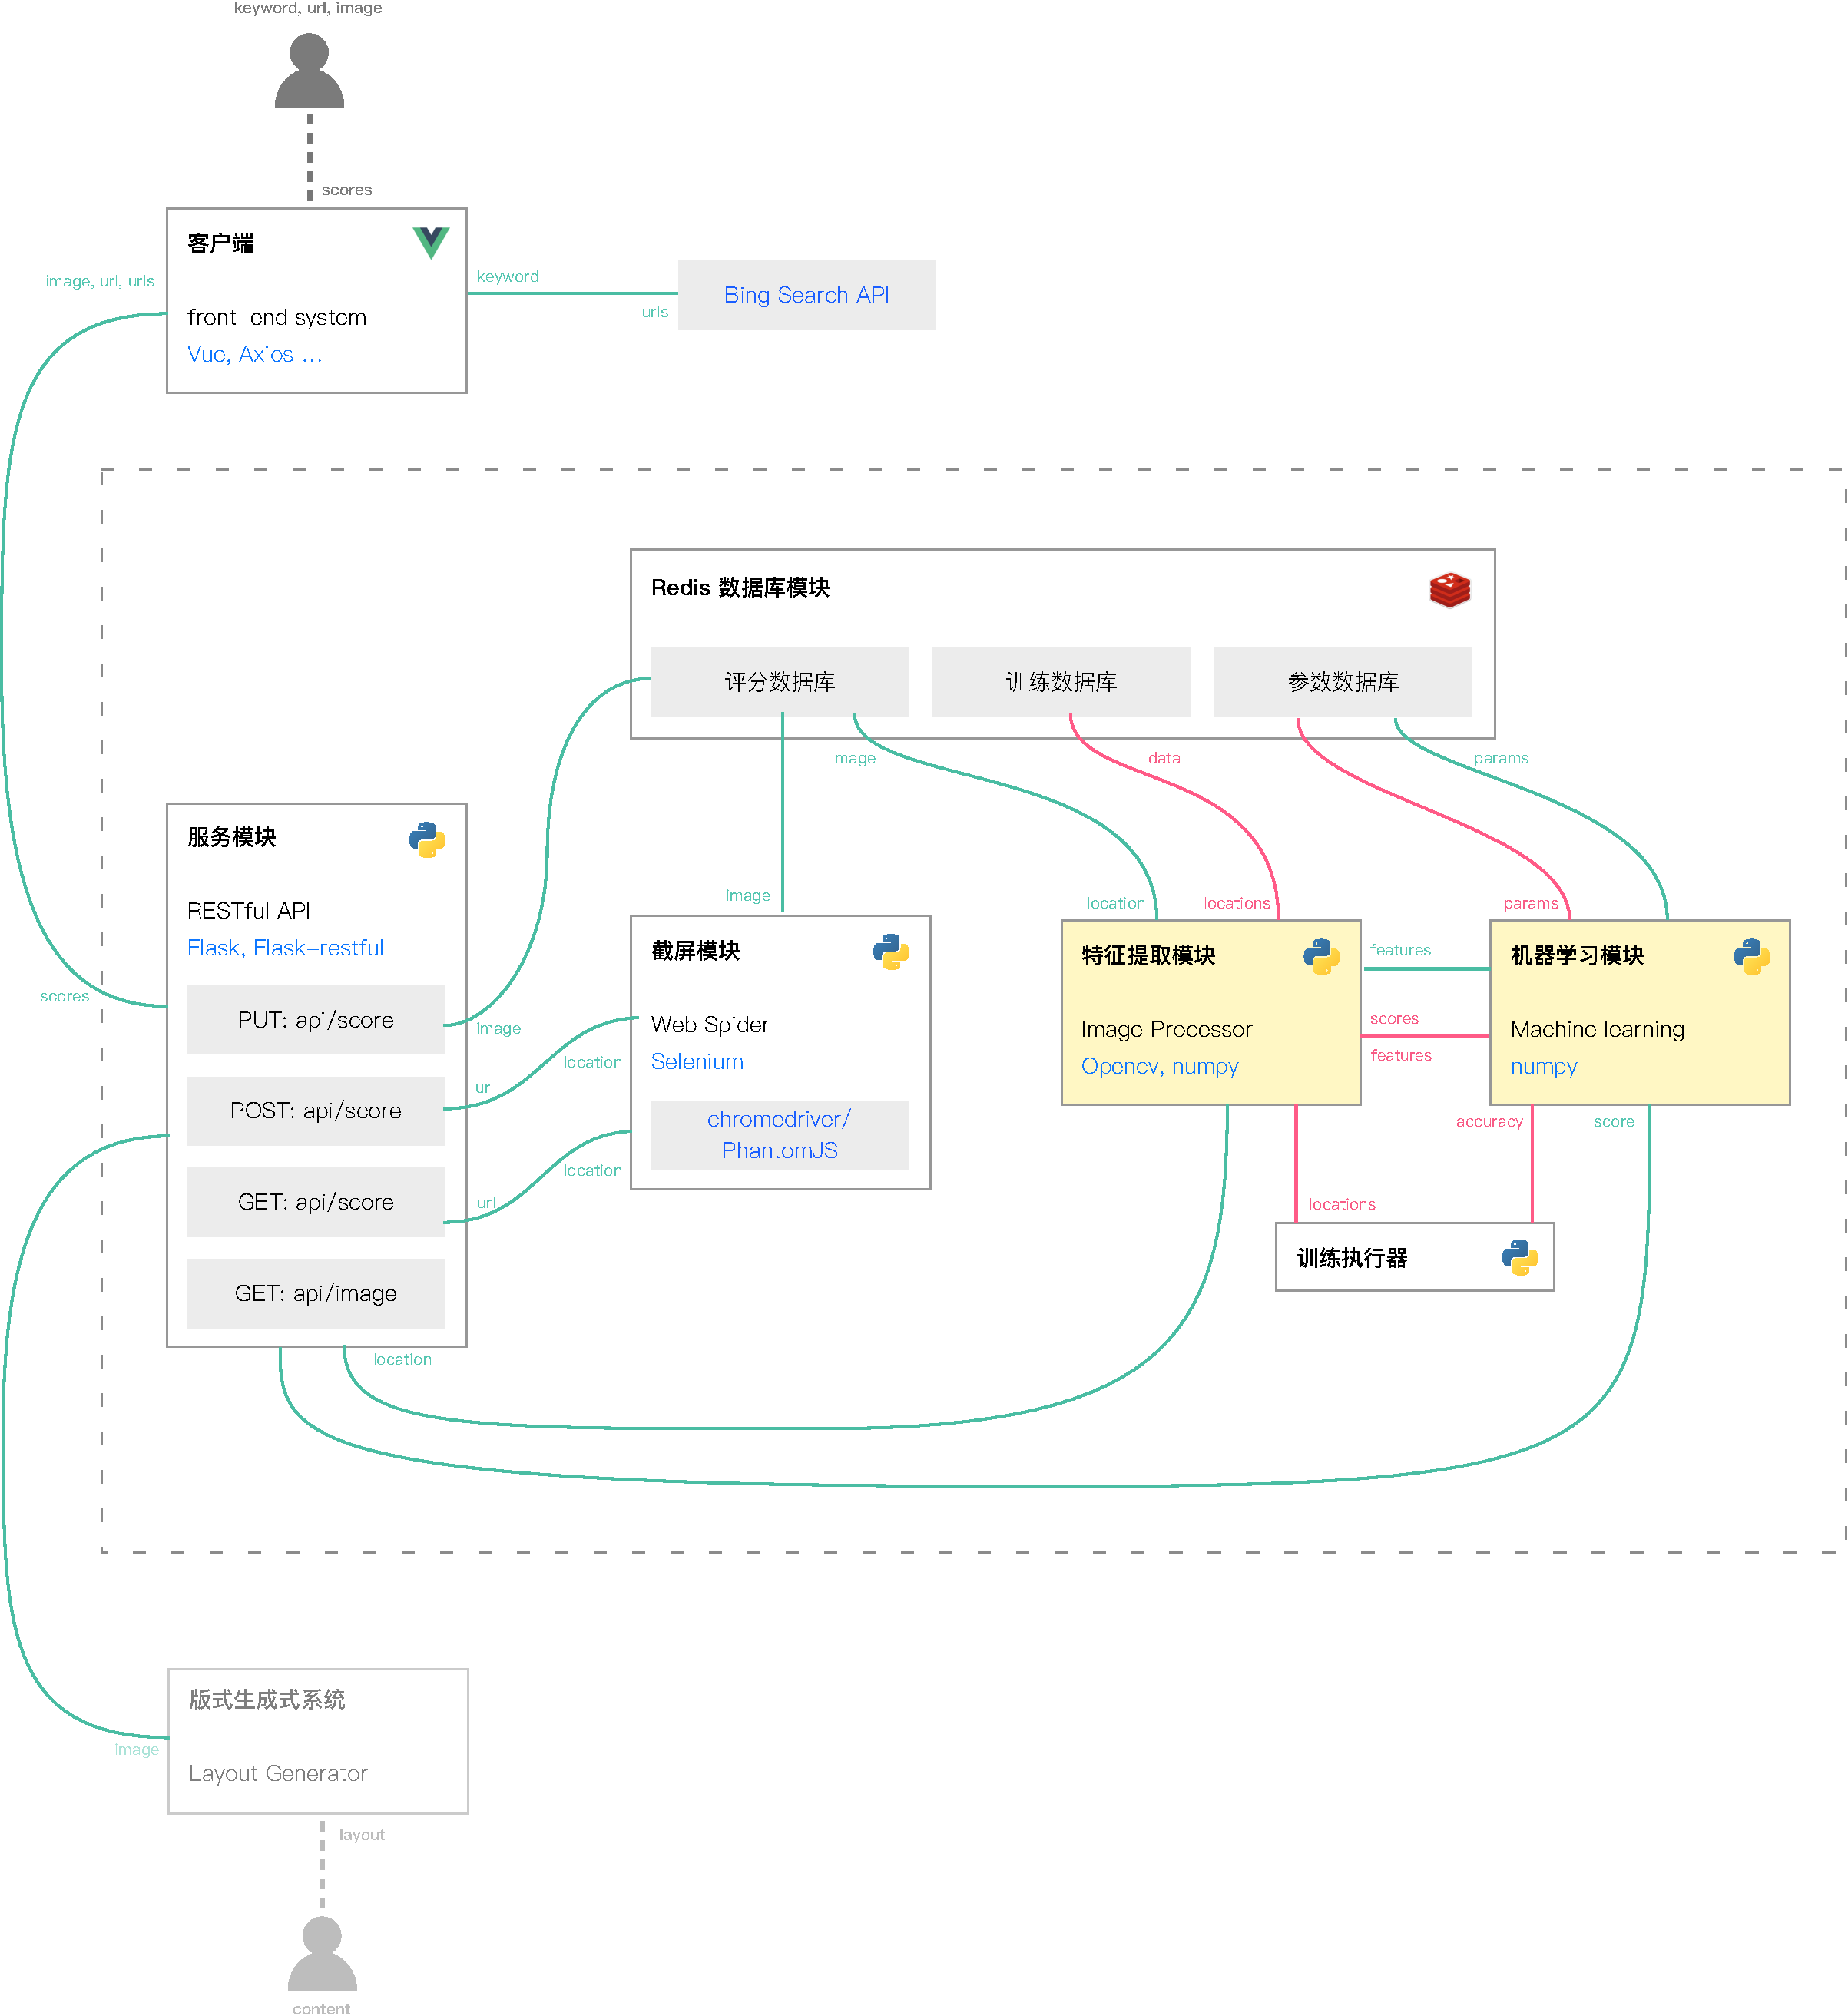
\includegraphics[width=\columnwidth]{fig/fig_sys_structure.pdf}
  \bicaption[fig:sys_struct]{评分系统的模块化架构}{评分系统的模块化架构,图解见图\ref{fig:sys_instruct}}{Fig}{the modular structure of the evaluating system}
\end{figure}
\subsection{模块化设计}

软件工程的模块化设计(Modular Design)是通过把系统划分成可以在不同系统中独立复用的模块(Modules)的设计模式。这些模块构成图状结构,在系统中仅仅通过约定好的接口(Interfaces)进行数据交换。模块化设计可以提高代码的复用率、提高系统对维护开发等过程造成的变化的适应能力\citen{Baldwin2000}。

\begin{figure}[H]
  \center
  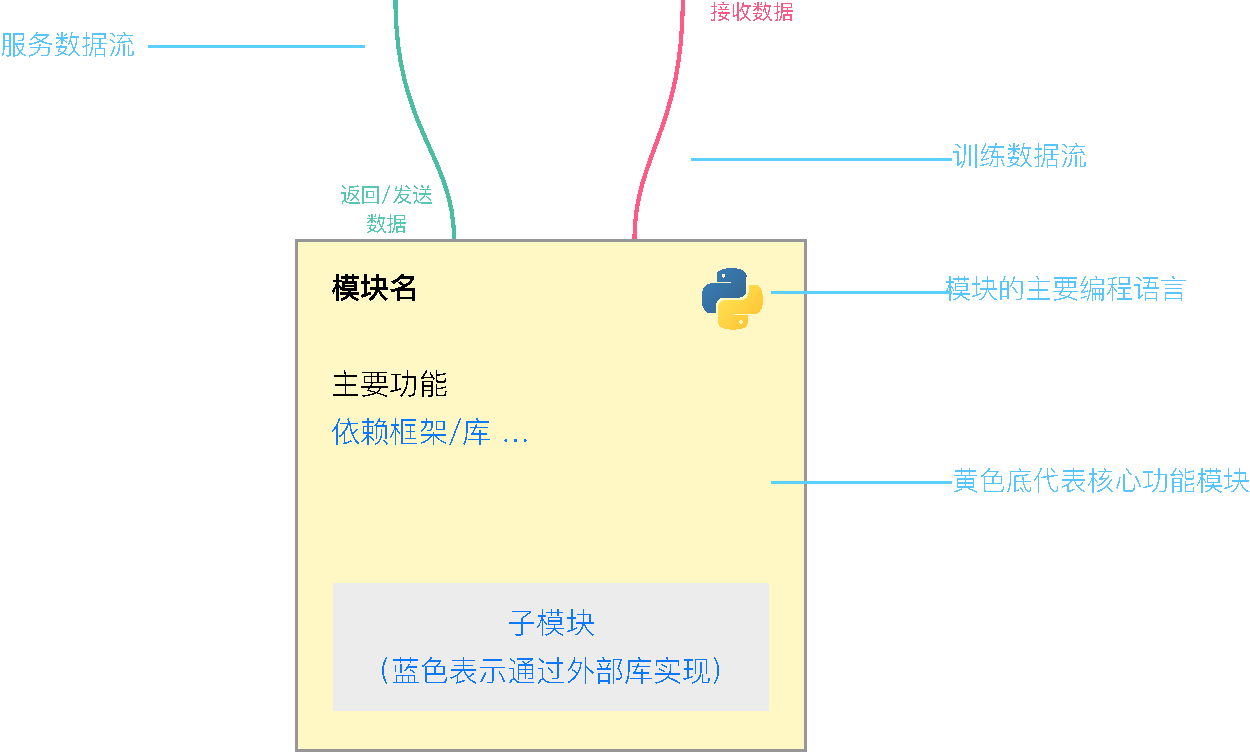
\includegraphics[width=0.6\columnwidth]{fig/fig_struct_instruction.pdf}
  \bicaption[fig:sys_instruct]{评分系统的模块图解}{评分系统的模块图解}{Fig}{the sketch map of a modular}
\end{figure}

图\ref{fig:sys_struct}表现了网页版式评分系统的模块架构。每一个实线矩形代表能够独立实现一项主要功能的模块,图\ref{fig:sys_instruct}说明了这些模块内的文字的含义。虚线矩形内框出的为网页版是美感评分系统,包含了与向外界提供HTTP服务的服务模块;对给定的url进行自动截图的截屏模块;用于管理数据的数据库模块;用于对图像提取特征的特征提取模块,用于进行机器学习的机器学习模块,以及用于驱动训练过程的训练模块。黄色背景的代表系统的核心模块。
虚线框的外部给出了网页版式评分系统的两种应用:上方是一个用户界面模块,展示了用户如何通过用户界面调用评分系统实现网页版式评分相关的需求,如:对关键词的搜索结果按照版式美感排序;上传一张网页图片获得其美感评分等,该模块的功能已经实现。下方是尚未一个实现的网页版式生成式系统,生成式系统可以通过调用评价模块来评价自己生成的网页排版,从而实现生成式的自动化设计,这部分功能尚待实现。

下面通过数据流和模块两部分来具体解释系统的运作方式和采用的技术。

\subsection{数据流}

\subsubsection{服务数据流}
服务数据流描述用户调用评分系统获取评分的过程。以用户对一个输入网页的url以获取网页版式评分的应用场景为例。用户向界面模块输入一个URL,界面模块将URL通过HTTP协议请求报表的形式发送给评分系统的服务模块。服务模块转发数据给截屏模块,截屏模块依照URL对网页进行截图,并将截图交给数据库,数据库储存成功后返还一个标志着截图的存储位置的键(key)给截屏模块,截屏模块转发键给特征提取模块,特征提取模块根据键向数据库获取图片并将提取完的特征向量返还给数据库储存,随后将键交给下游的机器学习模块,机器学习模块根据key向数据库获取特征和学习模型的参数进行评分,将评分一方面存数数据库,一方面返还给服务模块,标志着评分过程的结束。服务模块收到评分后再通过HTTP响应报表将分数发送给界面,界面将分数呈献给用户,就完成了整个服务数据流。

\subsubsection{训练数据流}
训练数据流描述系统内部的参数训过程。训练模块发起训练指令后,特征提取模块读取数据库训练数据集中的数据,开始特征提取,并存数训练数据集。机器学习模块读取这些提取完毕的特征进行模型训练,将训练完毕的模型参数存入数据库中专门的参数模块以供服务数据流调用。除了初始化参数数据库,训练数据流在日常也会不断受到来自外部的训练数据,发起训练过程,迭代更新模型参数以实现与时俱进的评价系统。

\subsection{模块}
\subsubsection{数据库(database)}
依赖:Redis

语言:Python,Redis

为了实现各个模块之间的功能性解耦,所有的模块之间均仅仅通过网页截图计算得到的键(key)来进行沟通,已完成制定的逻辑过程。而每个模块产生的数据,或是计算需要获得的数据都通过一个全局数据库实现读写。

数据采用noSQL的Redis数据库实现,总共划分为评分数据库(Eval\_db),训练数据库(Train\_db)以及参数数据库(Param\_db)三个部分。没个部分的数据通过键值对的嵌套结构进行存储。对于Redis的全部操作通过Python中实现的DB类来实现,包括了简单的增删改查和图像的编码解码等操作。

评分数据库负责缓存客户直接上传或者根据url截屏得到的图片。图片被转成base64编码格式。对base64编码通过哈希SHA1加密算法加密后取前8位,作为该图片保存的键(key)。采用哈希加密作为键的做法有诸多好处。哈希散列是一种对数据改变敏感的加密方式,只要图片数据发生改变,哈希散列就会完全不同。通过哈希散列验证数据是否损坏改变、快速反查上传的图片是否已经在数据库缓存等。图片信息以base64编码字符串的形式存储在数据库中该key下的字典的img字段中(在Redis中被称为哈希Hash)。字典还包含有feature(待计算的特征)字段特征和score字段(待计算的评分)。图\ref{fig:database}展示了存储一张图片内容的键值对的结构。评分数据库中的每个键值对被分别设置了自动释放时间(expire time),在保存24小时后会自动释放空间。

\begin{figure}[H]
  \center
  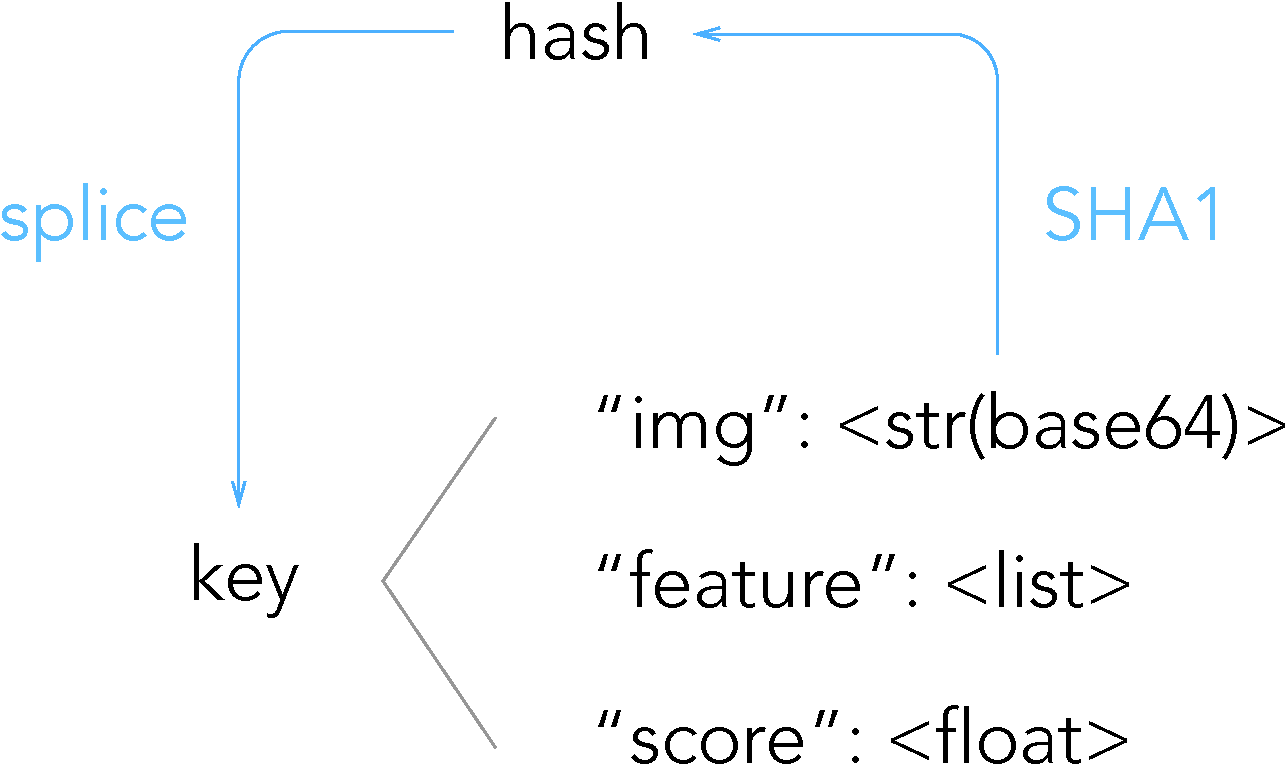
\includegraphics[width=0.4\columnwidth]{fig/fig_database.pdf}
  \bicaption[fig:database]{评分系统数据的键值对结构}{评分系统数据的键值对结构}{Fig}{the key-value hash structure stored in Redis database}
\end{figure}

训练数据库负责存储用于初始机器模型的训练的数据集。以与评分数据库中完全一样的键值对方式进行存储,只是字典中的score字段在初始的时候就已经被标定完毕。训练数据库的所有数据都永久保留,不设置释放时间。

参数数据库的内容很简单,保存了机器模型训练得到的参数。以本文中采用的logistic回归为例,参数以列表的格式存在params字段下。

\subsubsection{服务(server)}
依赖:Flask,Flask-restful

语言:Python

服务模块是与前端的通讯接口,监听前端的请求,并发起系统内部的服务数据流。为了实现对多种请求的响应,服务模块一共开通了如下的4个基于HTTP协议的接口:

\begin{itemize}
  \item 上传url获取评分和键:GET  /api/score
  \item 上传url列表获取评分和键列表:POST  /api/score
  \item 上传图片获取评分和键:PUT  /api/score
  \item 上传键获取图片:GET /api/img
\end{itemize}

实现技术上,服务模块依赖用于快速构建RESTful api的python框架Flask-RESTful。

\subsubsection{截图(screenshot)}

依赖:Selenium,PhantomJS,chromedriver

语言:Python

截图模块接收一个url,获取截图并存入数据库。为了保证网页的渲染效果,通过python爬虫框架Selenium调用chrome浏览器的内核chromedriver进行截屏,亦可调用不会显示浏览器界面的后台虚拟浏览器PhantomJS来截屏,实践表明与chromedriver的渲染效果别无二致。

\subsubsection{特征提取(extractor)}
依赖: cv2,numpy,Pillow

语言:python

特征提取器依照实验二中提取特征的方法进行特征提取并存入数据库。采用图像处理库opencv2和矩阵运算库numpy来实现。特征提取模块通过键向数据库模块获得已经解码完成图像文件,并借助python图形处理库(PIL,此处用Pillow替代)转成Image对象,交由基于opencv2进行图像处理和特征提取的操作。Opencv-pyhton2在数据格式和计算上完全依赖numpy进行,图像处理的关键算法则委托其C++内核进行运算。

\subsubsection{学习与评价(evaluator)}
依赖:Tensorflow,numpy

语言:python

学习与评价模块根据键向数据库获取图像特征和评分(对训练数据流)并进行学习或是评分。学习和评价过程依赖Google开源的Tensorflow机器学习框架实现。Tensorflow意为张量流,结合numpy的矩阵运算和相关模型的数学基础,他可以方便地通过python构建一个学习模型的图,并在外部通过更为底层的语言进行训练和计算,并可进行gpu加速。

\section{小结}
\label{sec:app-sum}
通过对训练集数据按照2:8的验证(Validation)训练(Training)比进行交叉,上述演示系统达到$83\%$的分类准确率。离实际应用尚有一定差距,但一定程度上进一步补充了实验一和实验二关于进化论美学和流畅理论的验证。
